\documentclass[toc=bibliographynumbered, liststotoc]{scrartcl} %mit [draft] vor den {} erreicht man, daß statt der Grafiken nur ein Rahmen in Größe der Grafik gezeichnet wird. Zusätzlich wird der Name der einzufügenden Datei in diesen Rahmen geschrieben]{book}
\usepackage[utf8]{inputenc}
\usepackage[T1]{fontenc}
\usepackage{lmodern}
%\usepackage[english,ngerman]{babel} %Deutsch als Hauptsprache, z.b. für Inhaltsverzeichnis etc.
\usepackage[ngerman,english]{babel} % Englisch als Hauptsprache!!!

\usepackage{graphicx}
\usepackage{xspace}
\usepackage{amstext}
\usepackage{amssymb}
\usepackage{setspace}
\doublespacing
\usepackage{longtable}
\usepackage{booktabs}


\usepackage[paper=a4paper,margin=2.5cm]{geometry}
\usepackage{helvet}
\renewcommand*{\familydefault}{\sfdefault} %gehört zum Font


\usepackage{here} %erzwingt Platzierung von Bildern ("H" bei Option)


\begin{document}

\begin{titlepage}
%\begin{figure}[t]
\begin{center}

\includegraphics[scale=0.65]{pics/hulogo.pdf}\\[1cm]

%\end{figure}
\textsc{\textbf{\normalsize LEBENSWISSENSCHAFTLICHE FAKULTÄT\\[0.2cm]  INSTITUT FÜR BIOLOGIE\\[1.5cm]
\LARGE MASTERARBEIT\\[0.5cm]
\normalsize ZUM ERWERB DES AKADEMISCHEN GRADES\\[0.5cm] MASTER OF SCIENCE\\[2cm]}
\normalfont %Kapitälchen deaktivieren
\textit{\large "Körpergrößentrends in fossilen Landschildkröten aus dem Neogen"\\[0.5cm]
"Body size trends in Neogene testudinid tortoises" }\\[2cm]
\small vorgelegt von\\[0.5cm] Julia Joos \\[0.2cm] geb. am 18.05.1991 in Freudenstadt \\[1cm] angefertigt in der Arbeitsgruppe Paläozoologie\\[0.2cm]
am Institut für Biologie/Museum für Naturkunde\\[1cm]
Berlin, im Septenber 2017}
\end{center}


\end{titlepage}


\tableofcontents
\listoffigures                         
\listoftables                     
\newpage
\section{Introduction}
\subsection{Body size evolution}

%Laurin, 2004
The body size of organisms has been of interest to researchers for a long time \citep{Haldane1928,Peters1983}. It is a universal trait, that can be easily measured and compared among different organisms \citep{.}. Furthermore, it is readily available for many animals in the fossil record which allows for comparison with extant species \citep{.}. A number of biotic and abiotic factors including habitat, resource availability, competition, climate and many more influence body size and it is linked to ecological and evolutionary processes \citep{Blackburn1994a,Blueweiss1978,Smith2009}.
%, for example \todo{example?!}.
Patterns of body size variation across spatial and/or temporal scales have been described for many animal groups and some have been summarised as ecological rules \citep{Millien2006,Angielczyk2015}.
%and many biogeographical rules concern body size evolution: 
Cope's rule describes the gradual within-lineage body size increase over time \citep{Cope1887}. According to the island rule large species become smaller on islands while small species often show an increase in body size \citep{Foster1964}. Bergmann's rule \citep{Bergmann1848} states that animals attain larger at higher latitudes, which can be considered a special case of the temperature-size rule, which predicts an increase in body size at lower temperatures \citep{AngillettaJr2004a}.
While such patterns have been well documented
%described in many animal groups and species 
\citep{Millien2006}, the underlying mechanisms might not be the same in all taxa and require further investigation \citep{Smith2009}.
The development of body size or any other trait over time can follow different evolutionary trajectories, that describe general trends of trait evolution. If a trait does not significantly change, it is described as stasis. If a trait does change, this change can either be directional, referred to as a generalized random walk, or non-directional, which is described as an unbiased random walk. Recently, new analytical tools have been developed, to be able to determine which evolutionary model fits the development of a trait, for example size trends, best over time \citep{Hunt2006,Hunt2015}.
Changes in body size on the clade level can either be due to selective forces acting on the whole clade (trends) or individual species being influenced by different causes (tendencies) \citep{Hunt2006}. A trend can be an increase or decrease in minimum, mean or maximum size and can be caused by differing speciation and extinction rates and therefore occur independently of tendencies \citep{Smith2016}. Maximum size, for example, is usually expected to increase without being selected for \citep{Smith2016}.

%Smith et al., 2016
%However, when patterns of size increase are examined within lower-level taxa (e.g., phyla, classes), the trends found there are generally more consistent with the null (Table 2)

%\todo{include evolutionary models here!!}


\subsection{Maximal body size - Megafauna}
Many taxa have a right-skewed body size distribution, which means that smaller body sizes are more abundant than large ones \citep{Blackburn1994a,Kozlowski2002,Lyons2008}. This raises the question of why organisms are a certain size, if there is an optimal body size for each organisms, why some species attain larger sizes than others and which 
structural, physical and physiological properties determine and limit minimum or maximum body size
%the maximum possible body size depends on, structurally, physically and physiologically 
\citep{Smith2009}.
%are distribution yA potential optimal body size and extreme body size - either large or small - are of particular interest to many researchers . 
A large body size is associated with certain advantages, e. g. decreased predation risk, higher fasting endurance, higher competitive ability, all of which results in a higher fitness \citep{.}.
On the other hand, there are some disadvantages to having a larger body size since usually a larger range size and more resources are needed and generation times are often longer \citep{.}.
%a lot of implications regarding resource availability, resilience, fecundity, 
%but it has also been debated whether larger body sizes may entail a higher risk of extinction (...).
In the history of Earth, animals have again and again attained very large body sizes, although patterns of when and how often maximum body size is achieved are inconsistent across time and different animal groups \citep{Smith2016}.
%(Also, different patterns in minimum size, which could be due to poorer preservation of smaller forms.)
Some famous examples of giant forms are the large insects from the Carboniferous/Permian period, the giant non-avian dinosaurs from the Jurassic/Triassic, the giant mammals from the Quatenary or today's largest animal, the blue whale \citep{.}.
%Giant animal forms are often intrigiung, because they usually present the upper limit of what is possibe physically, physiologically and structurally. 
%For example, the large insect (dragonflies etc.) from the Carbonian/Permian border (?) seem absolutely surreal to us as well as the later non-avian dinosaurs, which still fascinate many people. And today's largest animal, the blue whale, is of interest to many people.
Animals with a body mass exceeding 44 kg (or sometimes 10 kg \citep{Sandom2014}) are referred to as megafauna \citep{Barnosky2004, Rhodin2015}.
%Animals are considered megafauna, if their body mass/body length exceeds 44 kg \citep{Barnosky2004} .
%Large size can have many advantages but also some disadvantages.
%Especially the mammalian megafauna has been in the focus of research, wooly mammoths, giant sloths, waldelefanten?, etc.
It has been suggested, that large animals are more prone to extinction than smaller ones \citep{.}. Reasons for this may be that large species usually need more resources, have a larger range and longer generation times \citep{.}. 
During the Quaternary, a huge number of large mammals which were considered megafauna went extinct \citep{.}.
A number of causes for these extinction events have been discussed, but while a meteorite and disease were dismissed as possible causes due to lack of evidence \citep{.}, two possible scenarios are still under discussion: climate change and anthropogenic influence \citep{.}.
Some recent studies suggest that human influence has been the main driver of these extinctions of mammalian megafauna \citep{Barnosky2004,Sandom2014,Gibbons2004,Schuster2000}.

%- extinctions seem to be more size-biased in vertebrates

While the mammalian megafauna as well as their extinction %Pleistocene extinctions 
have been well investigated, the herpetofauna has also lost a considerable number of species during the Quaternary \citep{Blain2016}. 
For example, many turtle and tortoise species have gone extinct, among those quite a few large species \cite{Rhodin2015}.
In former times, giant tortoises were abundant on the continents as well as on many islands, whereas today giant tortoises are present only on two island regions in the tropics \citep{.}
% - the Galapagos islands and the West Indian islands
.


%Some basic questions deal with the issue of optimal body size: is there one for every organism and if so, how is it determined, how does it evolve?
%Animals --> magintudes of body size, many have their greatest body size right now, possible maximum has not been reached! BUT reptiles not


% Smith et al., 2016:
%For body size evolution in particular, the most commonly observed and documentable kind of trend—a rise in the maximum—does not by itself tell us much about underlying tendencies. Maxima are expected to increase even if no tendencies, no evolutionary forces, are present. Thus, we cannot infer the existence of a selective advantage of large size merely from an increase in the maximum.
%If a clade first evolves at a size close to the minimum size possible for a particular body plan or ecology and subsequent speciation events are random with respect to size (i.e., descendants are equally likely to be larger or smaller than their ancestors), thenmean size will increase, because the lower bound prevents the variance from increasing in the direction of smaller sizes. This is an example of a passive trend, one with no increasing tendency.
%A positive association between body size and extinction risk has been demonstrated for Pleistocene and living mammals (Lyons et al. 2004, Davidson et al. 2009), marine and fresh- water fishes (Olden et al. 2007), and birds (Boyer 2010). The association between body size and extinction risk is widely interpreted to result from the inverse association of body size with ecologically important traits such as population size, fecundity, and total resource requirements (Brown 1995).



%\subsection{Megfauna extinctions (mammals)}


%\subsection{Ectothermic megfauna}

%--> dinos BUT also giant tortoises


\subsection{Giant Tortoises - Testudinidae}
In the fossil record two clades of terrestrial tortoises have been identified, which both contained giant forms. One is the family Meiolaniidae, which occurred exclusively in Australia and is completely extinct nowadays \citep{.}. The other is the family Testudinidae, which comprises all extant terrestrial tortoises as well as many extinct or fossil taxa \citep{.}. The testudinids included giant forms and occurred on all continents but Australia \citep{.}.
Testudinidae have been known in the fossil record from the Eocene on, the earliest fossils stemming from Africa \citep{.}.
Body size played an important role in the earlier times of testudinid taxonomy \citep{.}. In the beginning, all tortoise fossils were assigned to the genus Testudo, but around the 20th century(??), tortoises were grouped into two clades based on body size. Large taxa were all assigned to the genus \textit{Geochelone}, while small tortoises were assigned to \textit{Testudo}.
Eventually, over the past few decades, the taxonomy has been revised for many regions, based on morphological and biogeographical clues \citep{.}. In the Americas, all tortoises are now referred to as either \textit{Hesperotestudo}, \textit{Gopherus} or \textit{Chelonoidis}, the latter contains all extant Galapagos giant tortoises \citep{.}. In Europe, the genus \textit{Cheirogaster} has been introduced but is currently being replaced by \textit{Titanochelon}, although not all species have been revised accordingly yet \citep{.}. Small species still belong to \textit{Testudo}, which contains the extant \textit{Testudo graeca}-group \citep{.}.
In Asia and Africa, the two current biodiversity hotspots for turtles and tortoises in general \citep{.}, many different taxa have now been differentiated \citep{.}.
In Asia, the genera \textit{Geochelone}, \textit{Indotestudo} and \textit{Manouria} are present \citep{.}. On mainland Africa there are seven extant genera: \textit{Homopus}, \textit{Psammobates}, \textit{Kinixys}, \textit{Malacochersus}, \textit{Chersina}, \textit{Stigmochelys} and \textit{Centrochelys}, the latter consisting of one species, \textit{Centrochelys sulcata}, which is the largest extant continental tortoise with a carapace length of about 80 cm \citep{.}. In the West Indian Islands (Madagascar, Seychelles, Aldabra etc.), there are three extant gerena, \textit{Astrochelys}, \textit{Pyxis} and the giant \textit{Aldabrachelys}, as well as the extinct \textit{Cylindraspis} \citep{.}.

On the contintents as well as remote islands giant tortoises exceeding carapace lengths of 2 m were abundant in former times and have frequently been found in fossil deposits \citep{.}. The presence of large tortoises on islands has been explained by their ability to float and to survive for months without water or food \citep{Gerlach2006, Patterson1973, Cheke2016}. 
%Cheke et al. 2016: Meilania also floated to islands!!

%The colonization of islands has been achieved by tortoises due to their resilience, they can cope without food or water for months (which is why they have been exploited by humans in the past --> whaling industry), their bouyancy. 

However, the abundance of giant tortoises on these remote oceanic islands along with their resilience and survivability without resources made them a very attractive food item for humans, especially in the whaling industry \citep{.}.
In addition to the exploitation of giant tortoises on islands, both small and large tortoises and turtles were also frequently eaten on the mainland \citep{.}.
%But also on the mainlands, and also small species have frequently been eaten, since turtles and tortoises 
Tortoises are easily captured, do not need a great amount of preparation before they can be cooked and can even be kept as a "staple" since they stay alive for quite a while withoud food or water \citep{Thompson2002,Thompson2014}. Intensive hunting and exploitation has been suggested to affect tortoise body size \citep{.} since larger individuals are more easily visible and yield more meat, they are more prone to exploitation than small ones \citep{Rhodin2015}. This may have lead to a decreased body size within a tortoise population, where tortoise consumption is common.
For this reason, tortoise body size has even been suggested as a proxy for human population size in some areas \citep{Steele2005,Stiner1999,Stiner2000}.
To this day, turtles and tortoises are still being eaten in some countries, although many are endangered \citep{.}.
Apart from anthropogenic influences, climate probably also affected tortoises \citep{.}. 
As ectotherms, turtles and tortoises are inherently more dependent on climate than endotherms \citep{.}. Especially large tortoises are very temperature-sensitive due to their unique physiology and morphology \citep{Swingland1979a, Swingland1979b}. In the fossil record, large tortoises are considered to be an indicator for mild winters in \citep{Hibbard1960,Schleich1981}, since they are thought to not have been able to dig themselves burrow for hibernation like modern Gopherus tortoises do (?? only in some places, I guess?)\citep{Carlson1999, Stojanov2009}. Additionally, giant tortoises run a high risk of overheating and display behavioral thermoregulation to keep their body temperature below a dangerous or even lethal value \citep{Sturbaum1982, Schleich1981}.
It has not been concluded with certainty, if anthropogenic influence or climate change or a mixture of both have caused the extinction of giant tortoises\citep{.}.

% \todo{over which time period??} 

%There, giant tortoises were abundant, just like they have been until a couple of hundreds of years ago on the Galapagos islands. On the West Indies, 2 species of Aldabrachelys actually went extinct in the past centuries (??)
 
%- mention Meiolania?
%- taxonomy
%- occurence
%- evolution/distribution
%- tortoises are temperature sensitive (?), well, giant tortoises seem to be.
%- have always been a preferred food source for humans (whaling industry)

\subsection{Body size trends in Testudinidae}

The aim of this work is to identify general body size distributions in tortoises (Testudinidae) on a global scale across the last 20 million years. Further, to investigate the general evolutionary mode of body size in testudinidae. 
%For this, the methods of Hunt (...) are used, which fit the mean trait, in this case carapace length, over time to different evolutionary models: either stasis, unbiased random walk or a generalized random walk. ... These mean and have been tested for ....????
Apart from that, focusing on giant tortoises, which were abundant in former times, but are extinct nowadays apart from a few remaining populations on tropical islands, to discuss where and when they occurred in the fossil record and which underlying reasons for the extinction of many giant forms have been stated in the literature.
Understanding how and why giant tortoises went extinct in the past, can hold valuable information for conservation work today. Many tortoise species are endangered and extinction rates have been especially high for insular species since the Pleistocene \citep{Rhodin2015}.

%- general body size distribution on a temporal and spatial scale
%- when/where did giant tortoises occurr, when/where did they disappear?
%- evolutionary mode of giant tortoises
%- how did they go extinct?


%- unbiased random walk: descendants are equally likely to be larger or smaller than their ancestors

\newpage
\section{Material \& Methods}

\subsection{Data collection}
I collected data on body size of fossil testudinids from the Upper Miocene until recent times. The body size data set includes 26 genera, comprising over 70 fossil and extant species. The majority of the data was obtained from the primary literature (\ref{TabS1}). To find relevant publications, I relied mostly on the references listed in FosFarBase (CITE), PDBD (cite), and "Fossil Turtle Checklist (CITE).
Furthermore, the FosFarBase provided fossil occurences of testudinids all over the world, including their exact localities and age (\ref{TabS2}), which were used to get an overview over the availability of body size data. 
For extant taxa, I measured dry material (n = 67) from the collection of the Museum für Naturkunde zu Berlin (MFN). In addition, body size data from the literature was included (\ref{TabS3}).

\subsection{Body size estimation}
Body size is reported as straight carapace length (SCL). Where SCL was not available from the primary literature, it was estimated either from plastron length (PL), femur length or humerus length (\ref{TabS1}). For carapace length estimations based on plastron length, the measurements from the MFN collection material was used to calculate the ratio between SCL and PL. Since the SC/PL ratio was similar for all species and genera, a single general ratio was calculated for all testudinids and hence used for the SCL estimations unless stated otherwise. For estimations based on humeri or femora, the ratios provided by Franz et al. (2001) were used.

TO DO: check Franz \& Quitmyer, 2005 again!! (CL regression)

\subsection{Analyses}
All subsequent analyses were performed with R (version ...), including the packages dplyr (cite) to manipulate the data and ggplot2 (cite) to create figures. Species Accumulation Curves were created to see if sample size sufficed. This was repeated on genus level, since genera of fossil testudinids are relatively well resolved by now whereas determination on the species level is still somewhat obscure in many cases, as quite some species were based on scarce material. Since the data set relies on literature, occurrences increase with each added reference and reach a maximum, when no new species/genera are added.



- only used samples > 11.000 mya?!

\subsection{Body size trends over time}
To investigate trends in body size over time, the R package paleoTS (cite) was used. Data were split into time bins according to the stratigraphic timescale (\ref{Tab1}). 
\newpage
\section{Results}

%read Willis et al., 2010 and Willis and Fortey, 2003 on use of paleontological data.

% read Thompson and Withers, 2003: Species Accumulation Curve
\subsection{Sample-based accumulation curves}
The sample-based accumulation curve (SAC) on the generic level shows a relatively low intial slope and a long upward slope to the asymptote, which does not reach full saturation (Fig. \ref{fig:SACGen}).
%Although the SAC does not completely plateau, considering the large area covered and the high number of rare genera in the dataset, it can be considered well enough sampled for our purposes.
In contrast, the species accumulation curves, both per reference and per locality, show only a slight initial increase and, for the same number of references/sampling units, are far from reaching an asymptote (Fig. \ref{fig:SACall} (a), (b)).
% DISCUSSION: as could be expected, since there are less genera than species \citep{Gotelli2001}. At a large geographic scale, it can be expected, that an asymptote is not reached \citep{Thompson2002}. Fig. \ref{fig:SACGen} corresponds to the shape one would expect, when there are many genera that are rare and only a few abundant ones. For the different continents, only Europe and Eurasia show some sort of "typical" SAC shape.
%%%____
% DISCUSSION ? 
%Since there are less genera than species, it is to be expected that genera reach an asymptote earlier than species.
%%%____
Accumulation curves for individual continents show that Europe reflects the trend of the overall dataset, with a long upward slope after the inflection point, whereas the other continents require further sampling (Fig. \ref{fig:SACall} (c) - (i)). For this reason, the timescale analysis was only conducted for Europe and Eurasia, but not for the other continents.

%--> genera sufficiently sampled, species not
%--> for genera, when splitting up continents only Europe and Eurasia are sampled well enough --> ask Johannes again, I feel like Asia is screwing up the results, would stick with Europe.
%--> maybe refer to table 20: overview over fossil genera per time bin??

%_______________________________________________________________________
\begin{figure}[htbp]
	\centering
	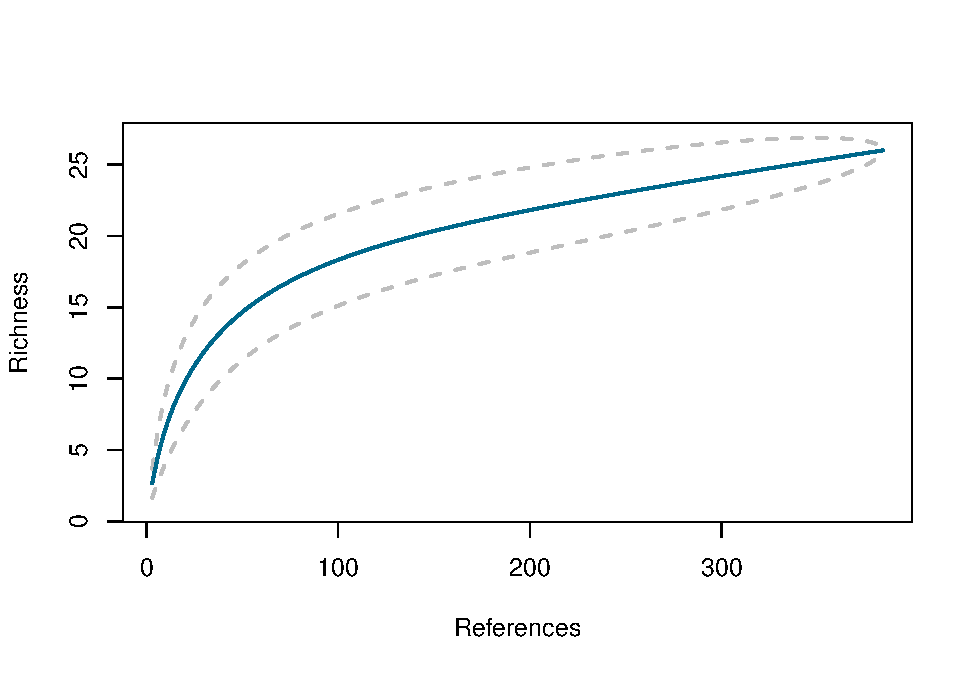
\includegraphics[width=0.8\textwidth]{MA_JJ_files/figure-latex/SACGenera-1.pdf}
	\caption[Sample-based accumulation curve on generic level]{Sample-based accumulation curve of fossil genera per reference. Dashed lines represent the confidence inteval.}
	\label{fig:SACGen}
\end{figure}


\FloatBarrier


%read: Smith and Lyons, 2010 (?) and Smith et al., 2016
%--> body size patterns (see also table 22, general statistics)

%data is bimodal (not normally distributed --> fig. ), still visible in pretty much all subgroups that you could split them into.
%as most animal groups/clades (?) right-skewed = smaller body size more frequent, BUT island species are left-skewed with more larger body sizes! (logtransformed data, skewness: negative for Zanclean, Messinian ??, insular, fossil-insular, but not modern-insular!!)
\subsection{Descriptive statistics}

The histograms indicate that testudinid body size is not normally distributed (Fig. \ref{fig:histAll}), which is supported by QQ-Plots for raw as well as log-transformed data (Fig. \ref{fig:NormDis}).

The body size distribution is moderately right-skewed (Table \ref{tab:stats}), with a higher frequency of smaller body sizes.
Body size ranges from a minimum of 80 mm to a maximum of 2500 mm for the entire data set. When comparing body sizes on a temporal scale, the minimum body size per stratigraphic stages excluding modern taxa ranges from 90 mm to 270 mm, while the maximum 1100 mm to 2500 mm. The highest maximum body size was observed in the fossil record from continental Europe (CL = 2500 mm).
%________________________________________________________________________

\begin{figure}[htbp]
	\centering
	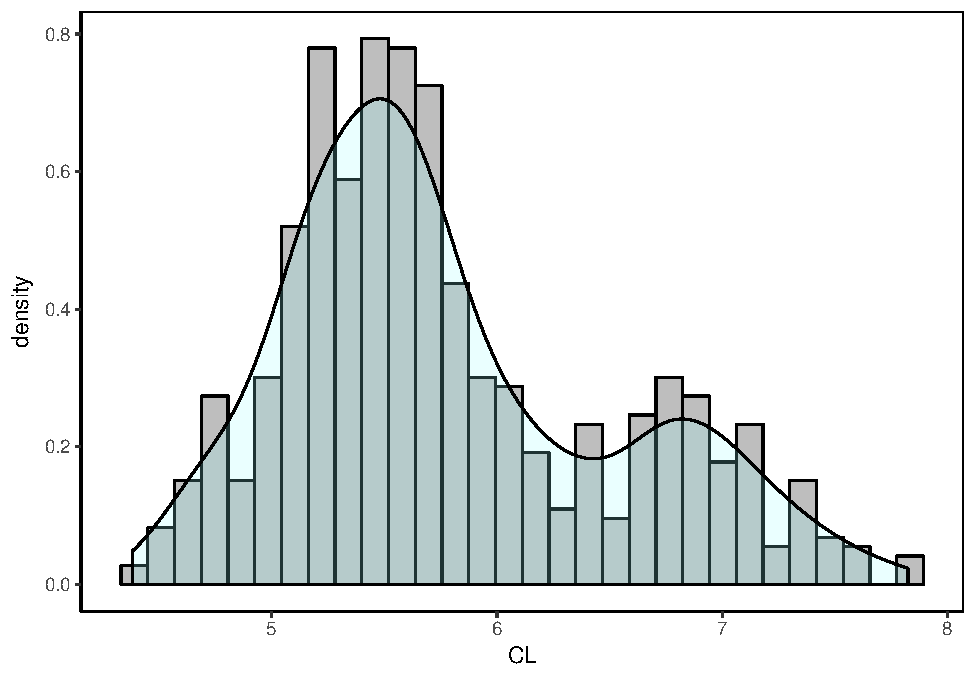
\includegraphics[width=0.8\textwidth]{MA_JJ_files/figure-latex/HistAll-1.pdf}
	\caption[CL distribution]{Body size distribution of complete data set. Bimodally distributed and right-skewed.}
	\label{fig:histAll}
\end{figure}

This pattern is also apparent when splitting the data set into fossil and modern taxa (Fig. \ref{fig:HistFMCI} (a)). Considering insularity, body size distribution is right-skewed for continental taxa, but left-skewed for insular species, meaning larger body size is more frequent than smaller body size on islands. Insular taxa are also left-skewed when only considering fossil taxa, but modern insular taxa have a skewness close to 0, indicating a symmetric distribution (Table \ref{tab:stats}).
Kurtosis suggests light tails with no/few outliers (kurtosis < 3) for insular and modern insular species, whereas continental species have a heavy tail (kurtosis > 3; Table \ref{tab:stats}).

\begin{center}
	\begin{figure}[htbp]
		\subfloat[Fossil vs. modern]{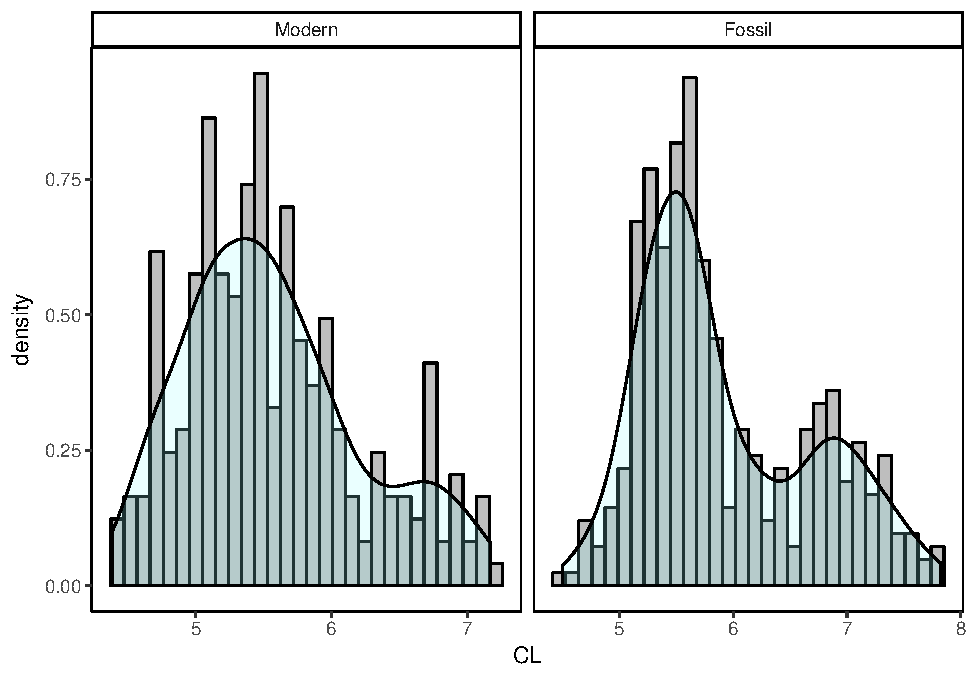
\includegraphics[scale=0.45]{MA_JJ_files/figure-latex/HistFosMo-1.pdf}}
		\subfloat[Continental vs. insular]{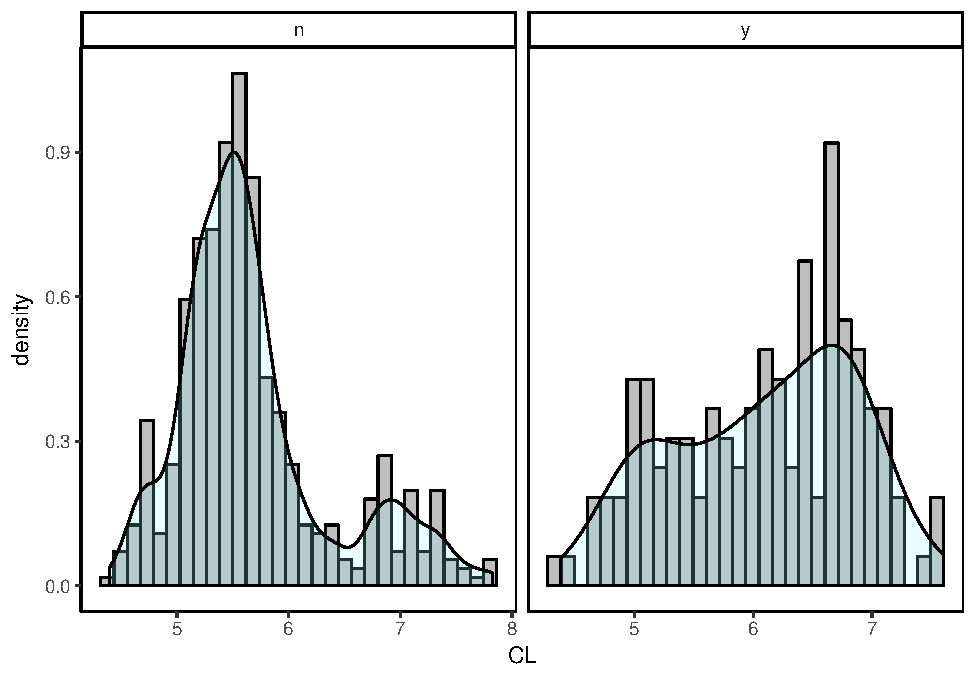
\includegraphics[scale=0.45]{MA_JJ_files/figure-latex/HistCI-1.pdf}}	
		\caption[Fossil vs. modern, continental vs. insular.]{Histograms for fossil vs. modern and continental vs. insular data.}
		\label{fig:HistFMCI}
	\end{figure}
\end{center}

The histograms show a bimodal distribution, wich is also apparent on most sublevels, except for modern insular species (Fig. \ref{fig:HistRest} (a)).
Body size distributions are similar, right-skewed and bimodal, for the four continents and reflect the overall trend (Fig. \ref{fig:HistRest} (b)).




\FloatBarrier

%__________________________



Mean body size differs significantly across time bins (Kruskal Wallis Test, $\chi^2$ = 71.441, P < 0.01; Fig. \ref{fig:boxBins}). 
The multiple comparison test showed that modern median body size is smaller than body size in the Upper Pleistocene. %(Wilcoxon Rank Sum Test, W = 3853.5, P < 0.01 )
There is no difference in body size within the Pleistocene %(Wilcoxon Rank Sum Test, P > 0.05)
and Pleistocene body size does not differ from body size in the Upper Miocene%(Wilcoxon Rank Sum Test, P > 0.05)
. Serravallian body size is smaller than Langhian body size in the Middle Miocene%(Wilcoxon Rank Sum Test, W = 45, P < 0.01)
, but Langhian body size is not different from Lower Miocene body size%(Wilcoxon Rank Sum Test, W = 311, P = 0.06)
.


%__________________________________________________________________________
\begin{figure}[hbtp]
	\centering
	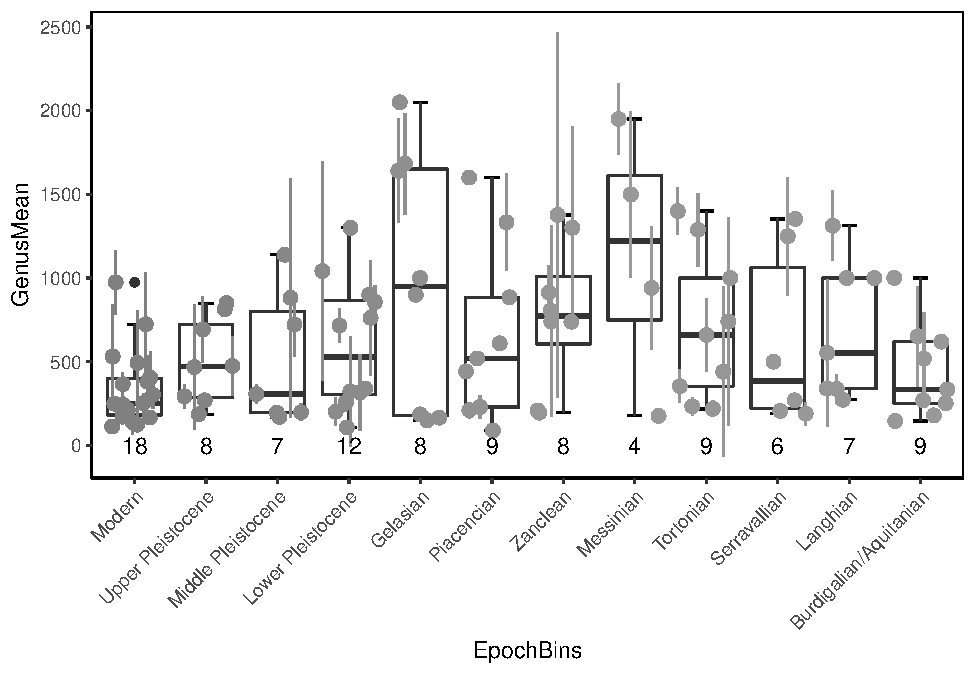
\includegraphics{MA_JJ_files/figure-latex/BPGBins-1.pdf}
	\caption{Boxplots of mean CL per time bin, including mean and sd CL for
		each genus (as pointrange).}
	\label{fig:boxBins}
\end{figure}

%\todo{random sampling necessary?}
% = 71.441, df = 11, p-value = 6.496e-11


%need statistics for boxplot!! kruskal-wallis-test plus post-hoc test (+ bonferroni correction?) or moving mean (faysal?)
%you can kind of see how the median increases and then decreases again
%(compare in order: Modern < Upper Pleistocene etc., do median and variance??)

% FOR ALL TIME STAGES

%	Kruskal-Wallis rank sum test

%data:  list(M, UPle, MPle, LPle, G, Pia, Z, Mess, Tort, S, L, BA)
%Kruskal-Wallis chi-squared = 71.441, df = 11, p-value = 6.496e-11

%Multiple comparison test after Kruskal-Wallis 
%p.value: 0.05 
%Comparisons
%obs.dif critical.dif difference
%Modern-Upper Pleistocene                  116.987013     93.54915       TRUE
%Modern-Middle Pleistocene                  80.140652     90.54349      FALSE
%Modern-Lower Pleistocene                   66.123604     87.87753      FALSE
%Modern-Gelasian                             1.627566    114.05459      FALSE
%Modern-Piacencian                         113.296537    136.11314      FALSE
%Modern-Zanclean                           205.945804    123.43828       TRUE
%Modern-Messinian                          137.122727    193.24680      FALSE
%Modern-Tortonian                           61.739394     96.96976      FALSE
%Modern-Serravallian                        21.764310    121.34770      FALSE
%Modern-Langhian                           202.487013    164.56067       TRUE
%Modern-Burdigalian/Aquitanian              70.472727    115.73561      FALSE
%Upper Pleistocene-Middle Pleistocene       36.846361    118.78423      FALSE
%Upper Pleistocene-Lower Pleistocene        50.863409    116.76486      FALSE
%Upper Pleistocene-Gelasian                115.359447    137.55006      FALSE
%Upper Pleistocene-Piacencian                3.690476    156.32773      FALSE
%Upper Pleistocene-Zanclean                 88.958791    145.42551      FALSE
%Upper Pleistocene-Messinian                20.135714    207.98052      FALSE
%Upper Pleistocene-Tortonian                55.247619    123.75260      FALSE
%Upper Pleistocene-Serravallian            138.751323    143.65527      FALSE
%Upper Pleistocene-Langhian                 85.500000    181.63641      FALSE
%Upper Pleistocene-Burdigalian/Aquitanian   46.514286    138.94713      FALSE
%Middle Pleistocene-Lower Pleistocene       14.017047    114.37094      FALSE
%Middle Pleistocene-Gelasian                78.513086    135.52379      FALSE
%Middle Pleistocene-Piacencian              33.155885    154.54785      FALSE
%Middle Pleistocene-Zanclean               125.805152    143.51048      FALSE
%Middle Pleistocene-Messinian               56.982075    206.64601      FALSE
%Middle Pleistocene-Tortonian               18.401258    121.49644      FALSE
%Middle Pleistocene-Serravallian           101.904962    141.71632      FALSE
%Middle Pleistocene-Langhian               122.346361    180.10681      FALSE
%Middle Pleistocene-Burdigalian/Aquitanian   9.667925    136.94153      FALSE
%Lower Pleistocene-Gelasian                 64.496038    133.75738      FALSE
%Lower Pleistocene-Piacencian               47.172932    153.00123      FALSE
%Lower Pleistocene-Zanclean                139.822200    141.84356      FALSE
%Lower Pleistocene-Messinian                70.999123    205.49188      FALSE
%Lower Pleistocene-Tortonian                 4.384211    119.52289      FALSE
%Lower Pleistocene-Serravallian             87.887914    140.02804      FALSE
%Lower Pleistocene-Langhian                136.363409    178.78144      FALSE
%Lower Pleistocene-Burdigalian/Aquitanian    4.349123    135.19364      FALSE
%Gelasian-Piacencian                       111.668971    169.39706      FALSE
%Gelasian-Zanclean                         204.318238    159.39129       TRUE
%Gelasian-Messinian                        135.495161    217.97454      FALSE
%Gelasian-Tortonian                         60.111828    139.89893      FALSE
%Gelasian-Serravallian                      23.391876    157.77782      FALSE
%Gelasian-Langhian                         200.859447    192.99946       TRUE
%Gelasian-Burdigalian/Aquitanian            68.845161    153.50345      FALSE
%Piacencian-Zanclean                        92.649267    175.85199      FALSE
%Piacencian-Messinian                       23.826190    230.28513      FALSE
%Piacencian-Tortonian                       51.557143    158.39839      FALSE
%Piacencian-Serravallian                   135.060847    174.39088      FALSE
%Piacencian-Langhian                        89.190476    206.80215      FALSE
%Piacencian-Burdigalian/Aquitanian          42.823810    170.53342      FALSE
%Zanclean-Messinian                         68.823077    223.02794      FALSE
%Zanclean-Tortonian                        144.206410    147.64914      FALSE
%Zanclean-Serravallian                     227.710114    164.68880       TRUE
%Zanclean-Langhian                           3.458791    198.68908      FALSE
%Zanclean-Burdigalian/Aquitanian           135.473077    160.59847      FALSE
%Messinian-Tortonian                        75.383333    209.54137      FALSE
%Messinian-Serravallian                    158.887037    221.87771      FALSE
%Messinian-Langhian                         65.364286    248.16258      FALSE
%Messinian-Burdigalian/Aquitanian           66.650000    218.85882      FALSE
%Tortonian-Serravallian                     83.503704    145.90588      FALSE
%Tortonian-Langhian                        140.747619    183.42158      FALSE
%Tortonian-Burdigalian/Aquitanian            8.733333    141.27276      FALSE
%Serravallian-Langhian                     224.251323    197.39708       TRUE
%Serravallian-Burdigalian/Aquitanian        92.237037    158.99725      FALSE
%Langhian-Burdigalian/Aquitanian           132.014286    193.99761      FALSE


% FOR MODERN - PLEISTOCENE - PLIOCENE - MIOCENE
%Kruskal-Wallis rank sum test

%data:  list(Modern, Plei, Plio, Mio)
%Kruskal-Wallis chi-squared = 37.764, df = 3, p-value = 3.172e-08


%Multiple comparison test after Kruskal-Wallis 
%p.value: 0.05 
%Comparisons
%obs.dif critical.dif difference
%Modern-Pleistocene   110.904114     49.80480       TRUE
%Modern-Pliocene       67.623302     58.35513       TRUE
%Modern-Miocene        64.510137     49.57182       TRUE
%Pleistocene-Pliocene  43.280812     64.36704      FALSE
%Pleistocene-Miocene   46.393977     56.52575      FALSE
%Pliocene-Miocene       3.113165     64.18694      FALSE



%__________________________________________________________________________
\begin{center}
	\begin{figure}[htbp]
		\subfloat[Fossil vs. modern]{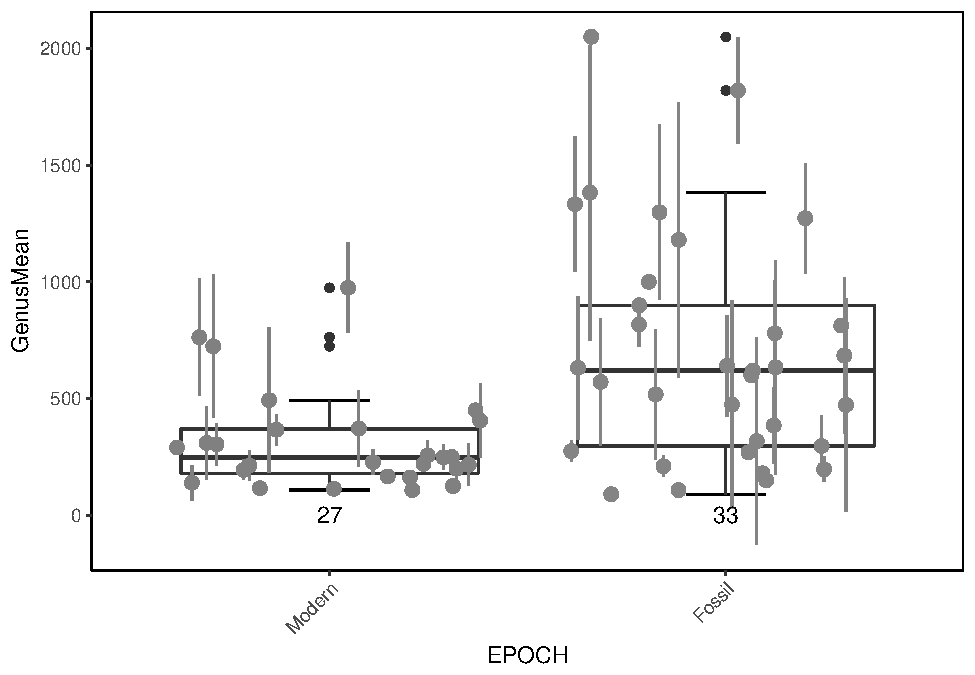
\includegraphics[scale=0.45]{MA_JJ_files/figure-latex/BPMF-1.pdf}}
		\subfloat[Continental vs. insular]{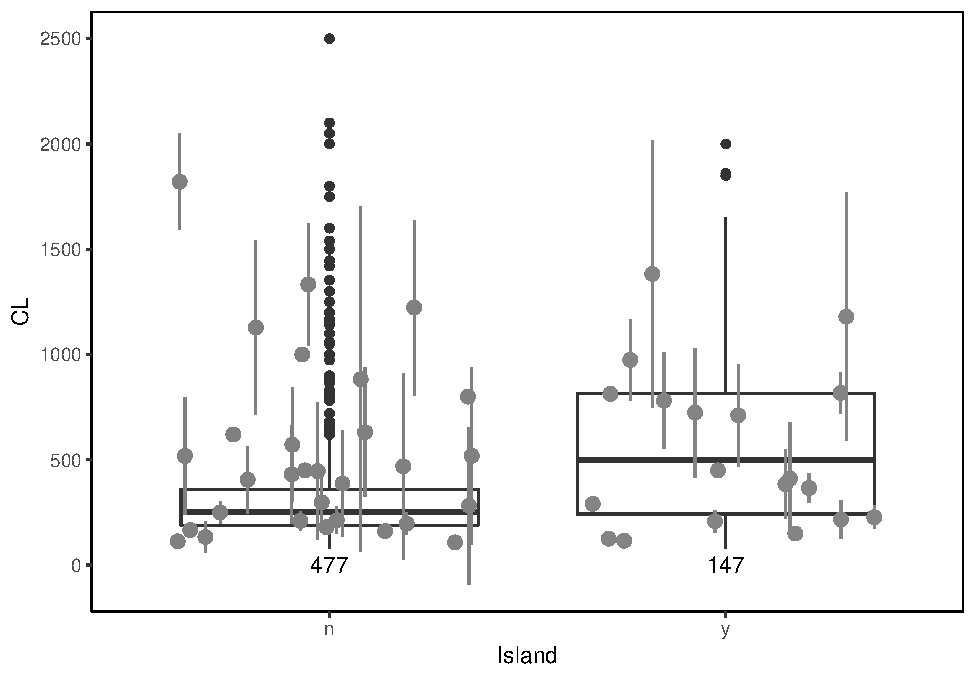
\includegraphics[scale=0.45]{MA_JJ_files/figure-latex/BPCI-1.pdf}}
		\caption{Boxplots of CL split into fossil vs. modern (a) and cotinental vs. insular (b)}
		\label{fig:boxFMCI}
	\end{figure}
\end{center}



Comparison of modern and fossil testudinids showed that modern tortoises are significantly smaller than fossil ones (Wilcoxon Rank Sum Test, W = 22318, P < 0.01; Fig. \ref{fig:boxFMCI}). Furthermore, continental testudinids are significantly smaller than insular taxa (Wilcoxon Rank Sum Test, W = 13854, P < 0.01; Fig. \ref{fig:boxFMCI}).
These results can even be considered in combination: modern continental taxa are smaller than fossil continental taxa (Wilcoxon Rank Sum Test, W = 8046, P < 0.01; Fig. \ref{BoxFoMCI}) and modern insular taxa are smaller than fossil insular taxa (Wilcoxon Rank Sum Test, W = 631.5, P < 0.01; Fig. \ref{BoxFoMCI}))

Finally, body size differs among continents (Kruskal Wallis Test, $\chi^2$ = 34.343, P < 0.01; Fig. \ref{fig:boxCon}). The multiple comparison test showed that African testudinids differ significantly from the other three continents in body size. American testudinid body size is comparable to that of Asia, but differs from those of Africa and Europe. Furthermore, Asian and European testidinids are similar in body size. %Since only Europe/Eurasia are well sampled, these relationships could change with further sampling. ??


\begin{figure}[htbp]
	\centering
	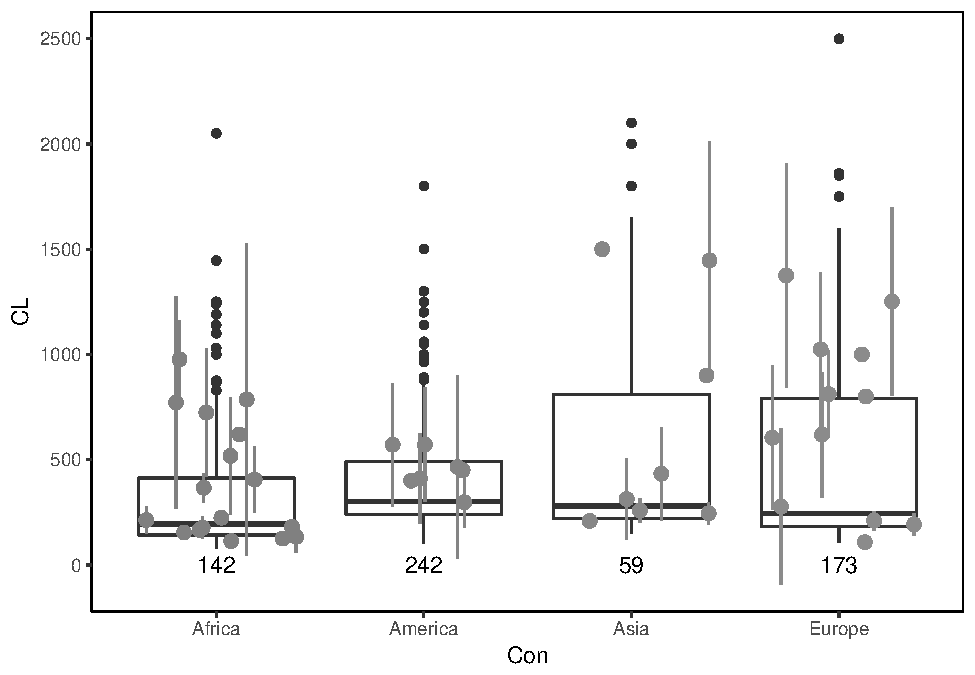
\includegraphics[width=0.75\textwidth]{MA_JJ_files/figure-latex/BPCon-1.pdf}
	\caption{Boxplot: body size on different continents, genera summarised}
	\label{fig:boxCon}
\end{figure}



\FloatBarrier
%__________________________________________________________________________

\subsection{paleoTS analysis}\label{paleots-analysis}




\subsubsection{complete dataset}\label{all-continental-and-insular}

Fitting of the three evolutionary models favoured stasis for the entire data set, although model support was only 51\,\% followed by 33\,\% support for the unbiased random walk (Fig. \ref{fig:pTSall}, Table \ref{tab:pTSall}). When solely considering continental genera, the best-fitting model was the unbiased random walk, but again not ideally supported with 55\,\% followed by a modest model support of 30\,\% for generalized random walk (Fig. \ref{fig:pTSC}, Table \ref{tab:pTSCEM}). In contrast, insular genera are best described by stasis, which was very well supported (100\,\%; Fig. \ref{fig:pTSI}, Table \ref{tab:pTSIEM})). 


\begin{figure}[H]
	\centering
	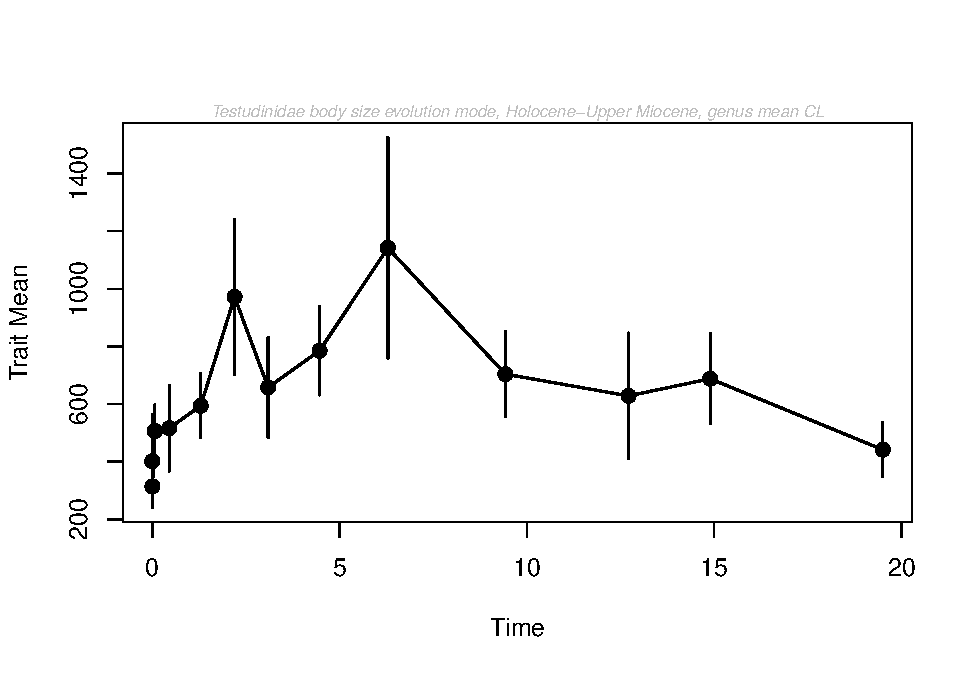
\includegraphics{MA_JJ_files/figure-latex/paleoTSAll-1.pdf}
	\caption{paleoTS plot with genus mean, all}
	\label{fig:pTSall}
\end{figure}

\begin{longtable}[]{@{}lrrrr@{}}
	\caption{Model-fitting results for testudinidae, genera,
		all}
	\label{tab:pTSallEM}\tabularnewline
	\toprule
	& logL & K & AICc & Akaike.wt\tabularnewline
	\midrule
	\endfirsthead
	\toprule
	& logL & K & AICc & Akaike.wt\tabularnewline
	\midrule
	\endhead
	GRW & -81.31790 & 2 & 167.9691 & 0.161\tabularnewline
	URW & -82.05721 & 1 & 166.5144 & 0.332\tabularnewline
	Stasis & -80.16802 & 2 & 165.6694 & 0.507\tabularnewline
	\bottomrule
\end{longtable}

\FloatBarrier
%__________________________________________________________________________

\subsubsection{continental dataset (excluding insular
	species)}\label{continental-excluding-insular-species}


\begin{figure}[H]
	\centering
	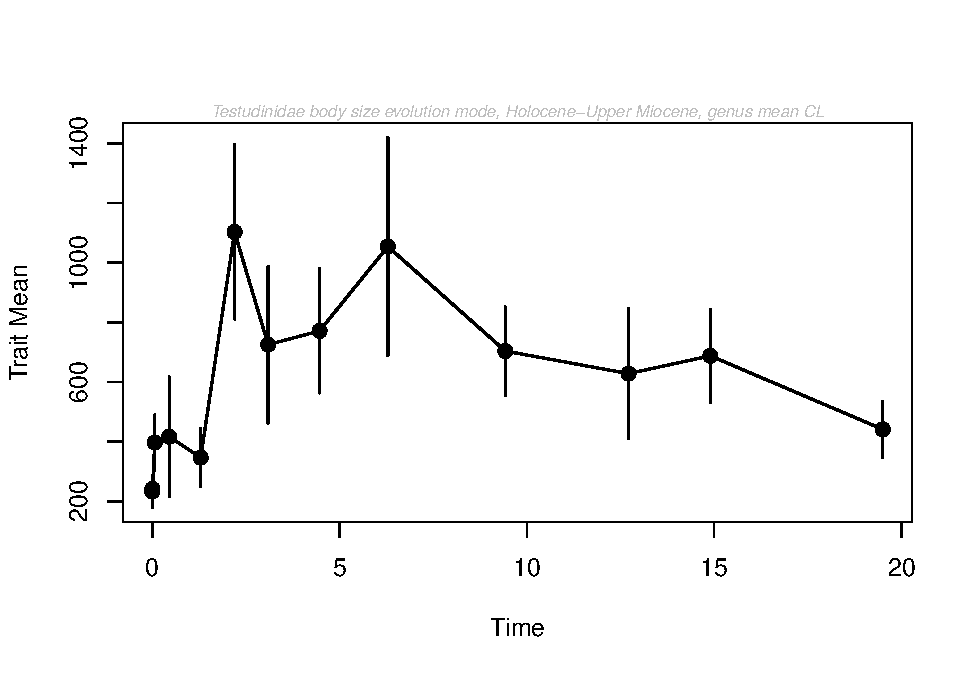
\includegraphics{MA_JJ_files/figure-latex/paleoTSC-1.pdf}
	\caption{paleoTS plot with genus mean, continental}
	\label{fig:pTSC}
\end{figure}

\begin{longtable}[]{@{}lrrrr@{}}
	\caption{Model-fitting results for testudinidae, genera,
		continental}
	\label{tab:pTSCEM}\tabularnewline
	\toprule
	& logL & K & AICc & Akaike.wt\tabularnewline
	\midrule
	\endfirsthead
	\toprule
	& logL & K & AICc & Akaike.wt\tabularnewline
	\midrule
	\endhead
	GRW & -82.26287 & 2 & 169.8591 & 0.300\tabularnewline
	URW & -83.12577 & 1 & 168.6515 & 0.548\tabularnewline
	Stasis & -82.93984 & 2 & 171.2130 & 0.152\tabularnewline
	\bottomrule
\end{longtable}


\FloatBarrier
%__________________________________________________________________________

\subsubsection{insular dataset (excluding
	continental)}\label{insular-excluding-continental}




\begin{figure}[H]
	\centering
	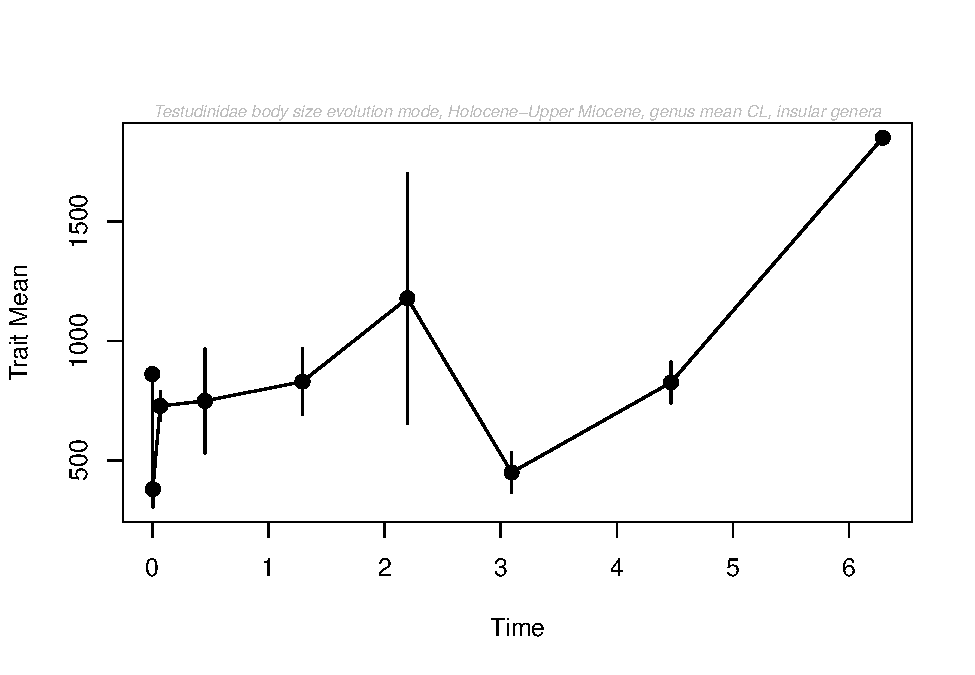
\includegraphics{MA_JJ_files/figure-latex/paleoTSI-1.pdf}
	\caption{paleoTS plot with genus mean, insular}
	\label{fig:pTSI}
\end{figure}

\begin{longtable}[]{@{}lrrrr@{}}
	\caption{Model-fitting results for testudinidae, genera,
		insular}
	\label{tab:pTSIEM}\tabularnewline
	\toprule
	& logL & K & AICc & Akaike.wt\tabularnewline
	\midrule
	\endfirsthead
	\toprule
	& logL & K & AICc & Akaike.wt\tabularnewline
	\midrule
	\endhead
	GRW & -68.57344 & 2 & 143.5469 & 0\tabularnewline
	URW & -75.76576 & 1 & 154.1982 & 0\tabularnewline
	Stasis & -60.41581 & 2 & 127.2316 & 1\tabularnewline
	\bottomrule
\end{longtable}

\FloatBarrier
%__________________________________________________________________________

\subsubsection{per continent}\label{per-continent}

\paragraph{Europe, genera}\label{europe-genera}

When repeating the analysis for European taxa only, all three groups -- complete, continental and insular data -- are best described by stasis with a model support between 92\,-\,99\,\% (Fig. \ref{fig:pTSEu}, \ref{fig:pTSEuC}, \ref{fig:pTSEuI}; Tables \ref{tab:pTSEuEM}, \ref{tab:pTSEuCEM}, \ref{tab:pTSEuIEM}).

\begin{figure}[H]
	\centering
	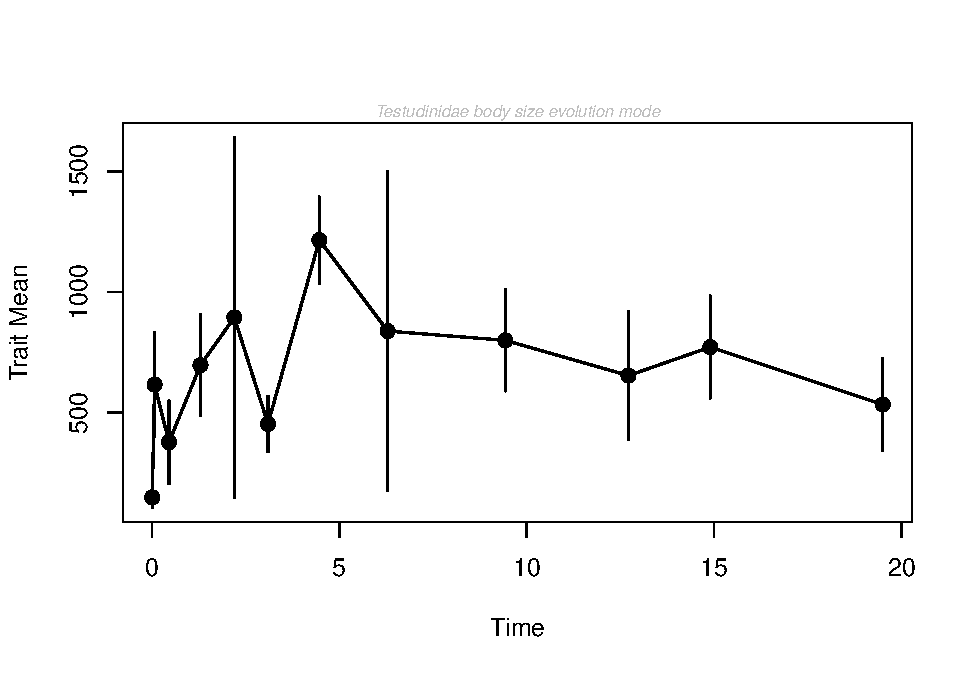
\includegraphics{MA_JJ_files/figure-latex/paleoTSEurope-1.pdf}
	\caption{Genera, Europe}
	\label{fig:pTSEu}
\end{figure}

\begin{longtable}[]{@{}lrrrr@{}}
	\caption{Model-fitting results for testudinidae, genera,
		Europe}
	\label{tab:pTSEuEM}\tabularnewline
	\toprule
	& logL & K & AICc & Akaike.wt\tabularnewline
	\midrule
	\endfirsthead
	\toprule
	& logL & K & AICc & Akaike.wt\tabularnewline
	\midrule
	\endhead
	GRW & -84.14010 & 2 & 173.7802 & 0.006\tabularnewline
	URW & -85.90727 & 1 & 174.2590 & 0.005\tabularnewline
	Stasis & -79.01365 & 2 & 163.5273 & 0.990\tabularnewline
	\bottomrule
\end{longtable}

\FloatBarrier
%__________________________________________________________________________



\paragraph{Eurasia,	genera}\label{eurasia-genera}


For Eurasia, the entire data as well as continental genera are best described by the unbiased random walk, although the model support is weak again. Continental species still have a better support (78\,\%; Fig. \ref{fig:pTSEsC}, Table \ref{tab:pTSEsCEM}) than all Eurasian data with only 56 \% (Fig. \ref{fig:pTSEs}, Table \ref{tab:pTSEsEM}). Insular Eurasian species, however, conform to stasis again, although with lower support values (68\,\%; Fig. \ref{fig:pTSEsI}, Table \ref{tab:pTSEsIEM}).



\begin{figure}[H]
	\centering
	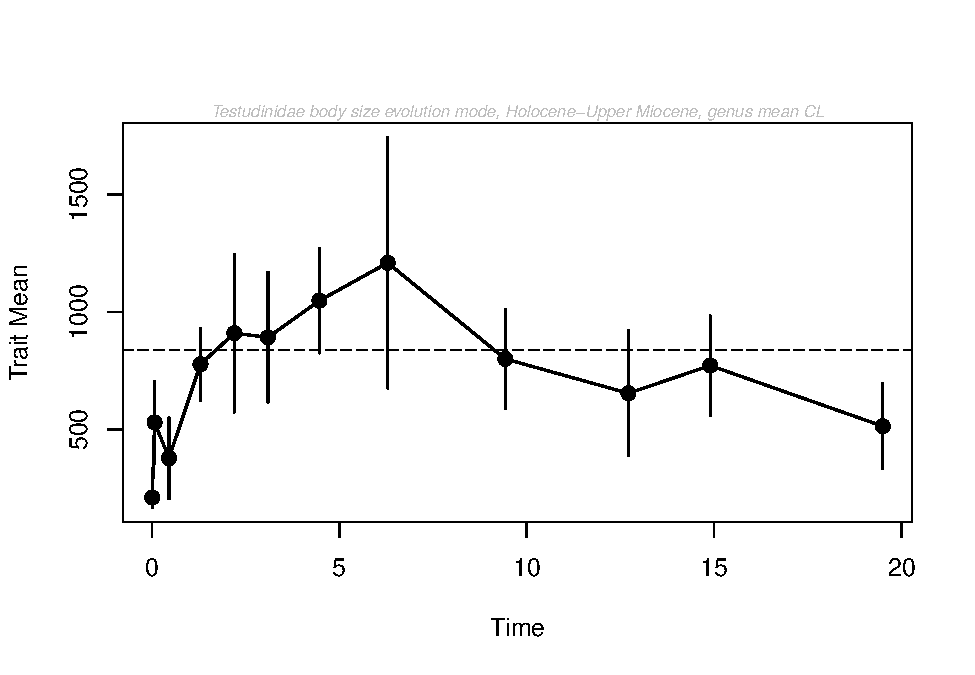
\includegraphics{MA_JJ_files/figure-latex/paleoTSEurasia-1.pdf}
	\caption{paleoTS, genera, Eurasia}
	\label{fig:pTSEs}
\end{figure}

\begin{longtable}[]{@{}lrrrr@{}}
	\caption{Model-fitting results for testudinidae, genera,
		Eurasia}
	\label{tab:pTSEsEM}\tabularnewline
	\toprule
	& logL & K & AICc & Akaike.wt\tabularnewline
	\midrule
	\endfirsthead
	\toprule
	& logL & K & AICc & Akaike.wt\tabularnewline
	\midrule
	\endhead
	GRW & -85.25195 & 2 & 175.8372 & 0.149\tabularnewline
	URW & -85.39072 & 1 & 173.1814 & 0.562\tabularnewline
	Stasis & -84.58890 & 2 & 174.5111 & 0.289\tabularnewline
	\bottomrule
\end{longtable}



\FloatBarrier
%__________________________________________________________________________




\end{document}